% ============================================================
%  Part 2: 产品线全景
% ============================================================

\section{产品线全景}

\subsection{产品线总览}

Astera Labs 当前拥有四条硬件产品线和一条软件平台产品线，见表~\ref{tab:products-all}：

\begin{table}[h]
    \centering
    \caption{Astera Labs 全产品线}
    \label{tab:products-all}
    \begin{tabular}{lllp{0.35\textwidth}}
        \toprule
        \textbf{产品} & \textbf{类型} & \textbf{协议/标准} & \textbf{核心价值} \\
        \midrule
        \rowcolor{blue!8}
        Scorpio X-Series & Smart Fabric Switch & Memory Semantic & GPU Scale-Up Fabric, 320 lanes \\
        \rowcolor{blue!8}
        Scorpio P-Series & Smart Fabric Switch & PCIe 6 & PCIe Fabric, 32–320 lanes \\
        \midrule
        Aries Retimer & Smart DSP Retimer & PCIe 6 / CXL 3.x & 信号再生, DSP 均衡 \\
        Aries Smart Cable & Active Cable Module & PCIe 6 / CXL 3.x & 7m 铜缆, 64 GT/s \\
        Aries Gearbox & Protocol Bridge & PCIe 6 $\leftrightarrow$ 5 & PCIe 代际过渡 \\
        \midrule
        Leo & CXL Memory Controller & CXL 1.1 & DDR5 内存扩展/池化 \\
        \midrule
        Taurus & Active Cable Module & Ethernet & 800G per link, 7m \\
        \midrule
        COSMOS & Software Platform & — & Telemetry, Fleet Mgmt, RAS \\
        \bottomrule
    \end{tabular}
\end{table}


\subsection{产品之间的战略关系}

产品路线图展现了一种典型的``平台扩展''策略——从一个技术核心（高速 SerDes/DSP）向多个方向辐射：

\begin{enumerate}
    \item \textbf{Aries Retimer} → 物理层基础。所有高速信号都需要它
    \item \textbf{Aries Smart Cable} → 将 Retimer 技术集成到 cable paddle card，实现``智能电缆''
    \item \textbf{Aries Gearbox} → 解决 PCIe 代际过渡的兼容性问题，保护客户现有的 NIC 投资
    \item \textbf{Scorpio P-Series} → 从 Retimer 向上扩展到交换，利用 PCIe 6 同一物理层
    \item \textbf{Scorpio X-Series} → 从标准 PCIe 扩展到 memory-semantic 协议，进入 GPU scale-up 领域
    \item \textbf{Leo} → 从连接扩展到内存，利用 CXL 协议做内存扩展
    \item \textbf{Taurus} → 从 PCIe 扩展到 Ethernet（scale-out），覆盖数据中心另一大连接领域
    \item \textbf{COSMOS} → 将所有硬件统一管理
\end{enumerate}

技术核心可归纳为三个 IP 支柱：
\begin{itemize}
    \item \textbf{SerDes/DSP IP}：Aries 系列的基础
    \item \textbf{Switching Fabric IP}：Scorpio 系列的基础
    \item \textbf{CXL Protocol IP}：Leo 的基础
\end{itemize}
COSMOS 是软件粘合剂，将所有硬件产品统一到单一管理平台。

\begin{figure}[htb]
    \centering
    \begin{tikzpicture}[
        node distance=0.4cm and 0.6cm,
        product/.style={rectangle, draw=darkblue, fill=blue!5, thick, minimum width=2.2cm, minimum height=0.8cm, align=center, rounded corners=3pt},
        platform/.style={rectangle, draw=darkgreen, fill=green!10, thick, minimum width=5.5cm, minimum height=0.8cm, align=center, rounded corners=3pt},
        arrow/.style={->, >=Stealth, thick, darkblue},
        arrow_sw/.style={->, >=Stealth, thick, darkgreen}
    ]
        % 第一行：Aries 产品
        \node[product] (ARIES_R) {Aries Retimer\\(SI 信号再生)};
        \node[product, right= 4cm of ARIES_R] (ARIES_G) {Aries Gearbox\\(PCIe 5$\leftrightarrow$6桥接)};

        % 第二行：居中于 ARIES_R 与 ARIES_G 之间
        \node[product, below=1cm] (ARIES_C) at ($(ARIES_R)!0.5!(ARIES_G)$) {Aries Smart Cable\\(智能有源电缆)};

        % 第三行：Scorpio 系列，位于 ARIES_C 下方两侧
        \node[product, below left= of ARIES_C] (SCORPIO_P) {Scorpio P-Series\\(PCIe 6 Fabric Switch)};
        \node[product, fill=darkred!15, below right= of ARIES_C] (SCORPIO_X) {Scorpio X-Series\\(Memory Semantic Fabric)};

        % 第四行：COSMOS 居中于 Scorpio 节点之间
        \node[platform, minimum width=5cm, below=1.5cm] (COSMOS) at ($(SCORPIO_P)!0.5!(SCORPIO_X)$) {COSMOS 软件平台 (统一管理)};

        % 第五行：Leo 与 Taurus 位于 COSMOS 下方两侧
        \node[product, below left= of COSMOS] (LEO) {Leo\\(CXL Memory Ctrl)};
        \node[product, below right= of COSMOS] (TAURUS) {Taurus\\(Ethernet Cable)};

        \draw[arrow_sw] (ARIES_R) -- (COSMOS);
        \draw[arrow_sw] (ARIES_C) -- (COSMOS);
        \draw[arrow_sw] (ARIES_G) -- (COSMOS);
        \draw[arrow_sw] (SCORPIO_P) -- (COSMOS);
        \draw[arrow_sw] (SCORPIO_X) -- (COSMOS);
        \draw[arrow_sw] (LEO) -- (COSMOS);
        \draw[arrow_sw] (TAURUS) -- (COSMOS);

        \draw[arrow, dashed, darkred] (ARIES_R) -- node[midway, left, font=\footnotesize] {DSP核心} (ARIES_C);
        \draw[arrow, dashed, darkred] (SCORPIO_P) -- node[midway, right, font=\footnotesize] {Scale-Up} (SCORPIO_X);
    \end{tikzpicture}
    \caption{产品拓扑关系图}
    \label{fig:product-topology}
\end{figure}

\subsection{产品在 AI 数据中心中的物理位置}

\begin{figure}[htb]
    \centering
    \begin{tikzpicture}[
        node distance=1.6cm and 1.2cm,
        gpu/.style={rectangle, draw=darkred, fill=red!10, minimum width=1.2cm, minimum height=0.7cm, align=center},
        nic/.style={rectangle, draw=darkgreen, fill=green!10, minimum width=1.2cm, minimum height=0.7cm, align=center},
        sw/.style={rectangle, draw=darkblue, fill=blue!10, minimum width=1.5cm, minimum height=0.7cm, align=center},
        ast/.style={rectangle, draw=gold, fill=yellow!15, thick, minimum width=1.8cm, minimum height=0.7cm, align=center},
        arrow/.style={->, >=Stealth, thick}
    ]
        \node[gpu] (GPU1) {GPU 0};
        \node[gpu, right=of GPU1] (GPU2) {GPU 1};
        \node[gpu, right=of GPU2] (GPU3) {GPU N};

        \node[ast, below=0.8cm of GPU2, minimum width=3.2cm] (SCORP) {Scorpio X-Series\\(Scale-Up Fabric)};

        \node[nic, below left=1.8cm of SCORP] (NIC1) {NIC 0};
        \node[nic, below right=1.8cm of SCORP] (NIC2) {NIC 1};

        \node[ast, below=0.5cm of NIC1, font=\footnotesize] (ARIES1) {Aries};
        \node[ast, below=0.5cm of NIC2, font=\footnotesize] (ARIES2) {Aries};

        \node[sw, below=0.8cm of ARIES1] (SW1) {Ethernet Switch};
        \node[sw, below=0.8cm of ARIES2] (SW2) {Ethernet Switch};
        \node[ast, right=of SW2, font=\footnotesize] (TAURUS_N) {Taurus};

        \node[rectangle, draw=purple, fill=purple!10, minimum width=2.5cm, minimum height=0.7cm, align=center, left=2.2cm of SCORP] (LEO_N) {Leo + DDR5\\(CXL Memory)};

        \draw[arrow] (GPU1) -- (SCORP);
        \draw[arrow] (GPU2) -- (SCORP);
        \draw[arrow] (GPU3) -- (SCORP);
        \draw[arrow] (SCORP) -- (NIC1);
        \draw[arrow] (SCORP) -- (NIC2);
        \draw[arrow] (NIC1) -- (ARIES1);
        \draw[arrow] (NIC2) -- (ARIES2);
        \draw[arrow] (ARIES1) -- (SW1);
        \draw[arrow] (ARIES2) -- (SW2);
        \draw[arrow] (SCORP) -- (LEO_N);
    \end{tikzpicture}
    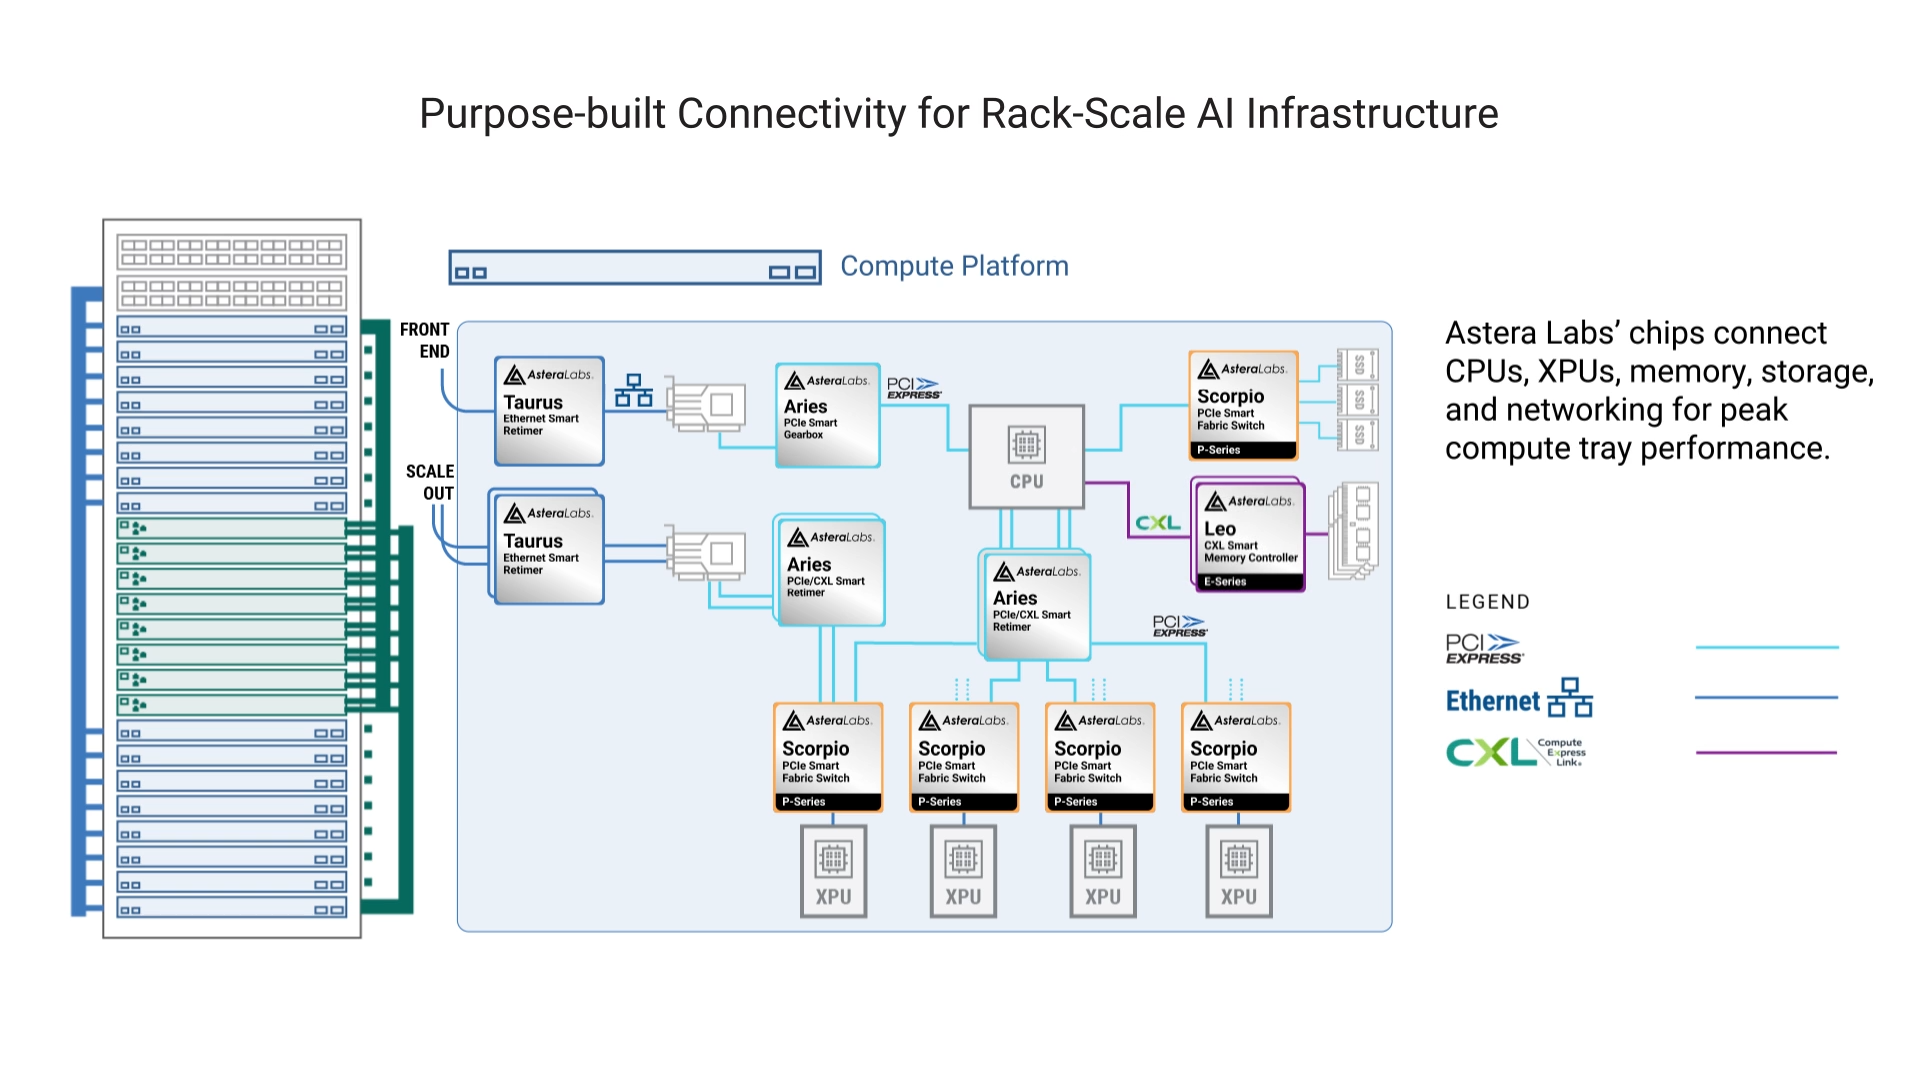
\includegraphics[width=0.9\textwidth]{./location.png}
    \caption{产品在 AI 数据中心中的物理部署位置}
    \label{fig:datacenter-location}
\end{figure}

\begin{itemize}
    \item \textbf{Scorpio X}：GPU-to-GPU Scale-Up（机箱/机架内）
    \item \textbf{Aries Retimer}：GPU/NIC 到外部连接（背板/电缆）
    \item \textbf{Taurus}：Scale-Out 网络（跨机架 Ethernet）
    \item \textbf{Leo}：CXL 内存扩展（GPU 共享内存池）
\end{itemize}
